\documentclass[1p]{elsarticle_modified}
%\bibliographystyle{elsarticle-num}

%\usepackage[colorlinks]{hyperref}
%\usepackage{abbrmath_seonhwa} %\Abb, \Ascr, \Acal ,\Abf, \Afrak
\usepackage{amsfonts}
\usepackage{amssymb}
\usepackage{amsmath}
\usepackage{amsthm}
\usepackage{scalefnt}
\usepackage{amsbsy}
\usepackage{kotex}
\usepackage{caption}
\usepackage{subfig}
\usepackage{color}
\usepackage{graphicx}
\usepackage{xcolor} %% white, black, red, green, blue, cyan, magenta, yellow
\usepackage{float}
\usepackage{setspace}
\usepackage{hyperref}

\usepackage{tikz}
\usetikzlibrary{arrows}

\usepackage{multirow}
\usepackage{array} % fixed length table
\usepackage{hhline}

%%%%%%%%%%%%%%%%%%%%%
\makeatletter
\renewcommand*\env@matrix[1][\arraystretch]{%
	\edef\arraystretch{#1}%
	\hskip -\arraycolsep
	\let\@ifnextchar\new@ifnextchar
	\array{*\c@MaxMatrixCols c}}
\makeatother %https://tex.stackexchange.com/questions/14071/how-can-i-increase-the-line-spacing-in-a-matrix
%%%%%%%%%%%%%%%

\usepackage[normalem]{ulem}

\newcommand{\msout}[1]{\ifmmode\text{\sout{\ensuremath{#1}}}\else\sout{#1}\fi}
%SOURCE: \msout is \stkout macro in https://tex.stackexchange.com/questions/20609/strikeout-in-math-mode

\newcommand{\cancel}[1]{
	\ifmmode
	{\color{red}\msout{#1}}
	\else
	{\color{red}\sout{#1}}
	\fi
}

\newcommand{\add}[1]{
	{\color{blue}\uwave{#1}}
}

\newcommand{\replace}[2]{
	\ifmmode
	{\color{red}\msout{#1}}{\color{blue}\uwave{#2}}
	\else
	{\color{red}\sout{#1}}{\color{blue}\uwave{#2}}
	\fi
}

\newcommand{\Sol}{\mathcal{S}} %segment
\newcommand{\D}{D} %diagram
\newcommand{\A}{\mathcal{A}} %arc


%%%%%%%%%%%%%%%%%%%%%%%%%%%%%5 test

\def\sl{\operatorname{\textup{SL}}(2,\Cbb)}
\def\psl{\operatorname{\textup{PSL}}(2,\Cbb)}
\def\quan{\mkern 1mu \triangleright \mkern 1mu}

\theoremstyle{definition}
\newtheorem{thm}{Theorem}[section]
\newtheorem{prop}[thm]{Proposition}
\newtheorem{lem}[thm]{Lemma}
\newtheorem{ques}[thm]{Question}
\newtheorem{cor}[thm]{Corollary}
\newtheorem{defn}[thm]{Definition}
\newtheorem{exam}[thm]{Example}
\newtheorem{rmk}[thm]{Remark}
\newtheorem{alg}[thm]{Algorithm}

\newcommand{\I}{\sqrt{-1}}
\begin{document}

%\begin{frontmatter}
%
%\title{Boundary parabolic representations of knots up to 8 crossings}
%
%%% Group authors per affiliation:
%\author{Yunhi Cho} 
%\address{Department of Mathematics, University of Seoul, Seoul, Korea}
%\ead{yhcho@uos.ac.kr}
%
%
%\author{Seonhwa Kim} %\fnref{s_kim}}
%\address{Center for Geometry and Physics, Institute for Basic Science, Pohang, 37673, Korea}
%\ead{ryeona17@ibs.re.kr}
%
%\author{Hyuk Kim}
%\address{Department of Mathematical Sciences, Seoul National University, Seoul 08826, Korea}
%\ead{hyukkim@snu.ac.kr}
%
%\author{Seokbeom Yoon}
%\address{Department of Mathematical Sciences, Seoul National University, Seoul, 08826,  Korea}
%\ead{sbyoon15@snu.ac.kr}
%
%\begin{abstract}
%We find all boundary parabolic representation of knots up to 8 crossings.
%
%\end{abstract}
%\begin{keyword}
%    \MSC[2010] 57M25 
%\end{keyword}
%
%\end{frontmatter}

%\linenumbers
%\tableofcontents
%
\newcommand\colored[1]{\textcolor{white}{\rule[-0.35ex]{0.8em}{1.4ex}}\kern-0.8em\color{red} #1}%
%\newcommand\colored[1]{\textcolor{white}{ #1}\kern-2.17ex	\textcolor{white}{ #1}\kern-1.81ex	\textcolor{white}{ #1}\kern-2.15ex\color{red}#1	}

{\Large $\underline{12n_{0445}~(K12n_{0445})}$}

\setlength{\tabcolsep}{10pt}
\renewcommand{\arraystretch}{1.6}
\vspace{1cm}\begin{tabular}{m{100pt}>{\centering\arraybackslash}m{274pt}}
\multirow{5}{120pt}{
	\centering
	\includegraphics[width=112pt]{../../../GIT/diagram.site/Diagrams/png/2534_12n_0445.png}\\
\ \ \ A knot diagram\footnotemark}&
\allowdisplaybreaks
\textbf{Linearized knot diagam} \\
\cline{2-2}
 &
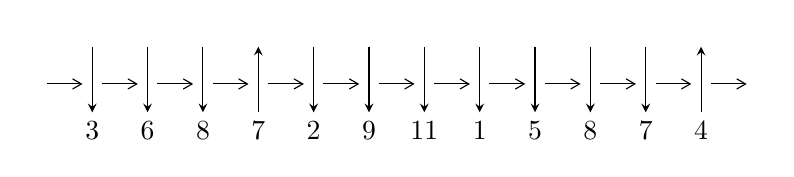
\begin{tikzpicture}[x=20pt, y=17pt]
	% nodes
	\node (C0) at (0, 0) {};
	\node (C1) at (1, 0) {};
	\node (C1U) at (1, +1) {};
	\node (C1D) at (1, -1) {3};

	\node (C2) at (2, 0) {};
	\node (C2U) at (2, +1) {};
	\node (C2D) at (2, -1) {6};

	\node (C3) at (3, 0) {};
	\node (C3U) at (3, +1) {};
	\node (C3D) at (3, -1) {8};

	\node (C4) at (4, 0) {};
	\node (C4U) at (4, +1) {};
	\node (C4D) at (4, -1) {7};

	\node (C5) at (5, 0) {};
	\node (C5U) at (5, +1) {};
	\node (C5D) at (5, -1) {2};

	\node (C6) at (6, 0) {};
	\node (C6U) at (6, +1) {};
	\node (C6D) at (6, -1) {9};

	\node (C7) at (7, 0) {};
	\node (C7U) at (7, +1) {};
	\node (C7D) at (7, -1) {11};

	\node (C8) at (8, 0) {};
	\node (C8U) at (8, +1) {};
	\node (C8D) at (8, -1) {1};

	\node (C9) at (9, 0) {};
	\node (C9U) at (9, +1) {};
	\node (C9D) at (9, -1) {5};

	\node (C10) at (10, 0) {};
	\node (C10U) at (10, +1) {};
	\node (C10D) at (10, -1) {8};

	\node (C11) at (11, 0) {};
	\node (C11U) at (11, +1) {};
	\node (C11D) at (11, -1) {7};

	\node (C12) at (12, 0) {};
	\node (C12U) at (12, +1) {};
	\node (C12D) at (12, -1) {4};
	\node (C13) at (13, 0) {};

	% arrows
	\draw[->,>={angle 60}]
	(C0) edge (C1) (C1) edge (C2) (C2) edge (C3) (C3) edge (C4) (C4) edge (C5) (C5) edge (C6) (C6) edge (C7) (C7) edge (C8) (C8) edge (C9) (C9) edge (C10) (C10) edge (C11) (C11) edge (C12) (C12) edge (C13) ;	\draw[->,>=stealth]
	(C1U) edge (C1D) (C2U) edge (C2D) (C3U) edge (C3D) (C4D) edge (C4U) (C5U) edge (C5D) (C6U) edge (C6D) (C7U) edge (C7D) (C8U) edge (C8D) (C9U) edge (C9D) (C10U) edge (C10D) (C11U) edge (C11D) (C12D) edge (C12U) ;
	\end{tikzpicture} \\
\hhline{~~} \\& 
\textbf{Solving Sequence} \\ \cline{2-2} 
 &
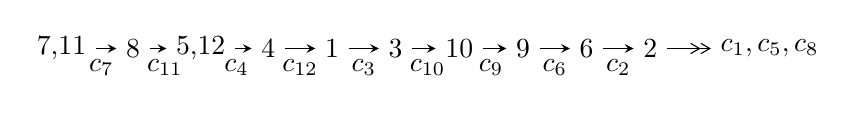
\begin{tikzpicture}[x=23pt, y=7pt]
	% node
	\node (A0) at (-1/8, 0) {7,11};
	\node (A1) at (1, 0) {8};
	\node (A2) at (33/16, 0) {5,12};
	\node (A3) at (25/8, 0) {4};
	\node (A4) at (33/8, 0) {1};
	\node (A5) at (41/8, 0) {3};
	\node (A6) at (49/8, 0) {10};
	\node (A7) at (57/8, 0) {9};
	\node (A8) at (65/8, 0) {6};
	\node (A9) at (73/8, 0) {2};
	\node (C1) at (1/2, -1) {$c_{7}$};
	\node (C2) at (3/2, -1) {$c_{11}$};
	\node (C3) at (21/8, -1) {$c_{4}$};
	\node (C4) at (29/8, -1) {$c_{12}$};
	\node (C5) at (37/8, -1) {$c_{3}$};
	\node (C6) at (45/8, -1) {$c_{10}$};
	\node (C7) at (53/8, -1) {$c_{9}$};
	\node (C8) at (61/8, -1) {$c_{6}$};
	\node (C9) at (69/8, -1) {$c_{2}$};
	\node (A10) at (11, 0) {$c_{1},c_{5},c_{8}$};

	% edge
	\draw[->,>=stealth]	
	(A0) edge (A1) (A1) edge (A2) (A2) edge (A3) (A3) edge (A4) (A4) edge (A5) (A5) edge (A6) (A6) edge (A7) (A7) edge (A8) (A8) edge (A9) ;
	\draw[->>,>={angle 60}]	
	(A9) edge (A10);
\end{tikzpicture} \\ 

\end{tabular} \\

\footnotetext{
The image of knot diagram is generated by the software ``\textbf{Draw programme}" developed by Andrew Bartholomew(\url{http://www.layer8.co.uk/maths/draw/index.htm\#Running-draw}), where we modified some parts for our purpose(\url{https://github.com/CATsTAILs/LinksPainter}).
}\phantom \\ \newline 
\centering \textbf{Ideals for irreducible components\footnotemark of $X_{\text{par}}$} 
 
\begin{align*}
I^u_{1}&=\langle 
4.88127\times10^{25} u^{40}-6.12725\times10^{26} u^{39}+\cdots+1.13889\times10^{27} b+1.45283\times10^{27},\\
\phantom{I^u_{1}}&\phantom{= \langle  }-1.45283\times10^{27} u^{40}-1.60788\times10^{28} u^{39}+\cdots+2.27778\times10^{27} a+3.79150\times10^{27},\;u^{41}+11 u^{40}+\cdots+u-2\rangle \\
I^u_{2}&=\langle 
-2 u^{21}+19 u^{20}+\cdots+b-1,\;-2 u^{21} a-3 u^{21}+\cdots+34 a-19,\;u^{22}-9 u^{21}+\cdots- u+2\rangle \\
I^u_{3}&=\langle 
u^{18}-8 u^{17}+\cdots+b+5,\;5 u^{18}-37 u^{17}+\cdots+3 a+11,\;u^{19}-8 u^{18}+\cdots+22 u-3\rangle \\
\\
I^v_{1}&=\langle 
a,\;b+v,\;v^2- v+1\rangle \\
\end{align*}
\raggedright * 4 irreducible components of $\dim_{\mathbb{C}}=0$, with total 106 representations.\\
\footnotetext{All coefficients of polynomials are rational numbers. But the coefficients are sometimes approximated in decimal forms when there is not enough margin.}
\newpage
\renewcommand{\arraystretch}{1}
\centering \section*{I. $I^u_{1}= \langle 4.88\times10^{25} u^{40}-6.13\times10^{26} u^{39}+\cdots+1.14\times10^{27} b+1.45\times10^{27},\;-1.45\times10^{27} u^{40}-1.61\times10^{28} u^{39}+\cdots+2.28\times10^{27} a+3.79\times10^{27},\;u^{41}+11 u^{40}+\cdots+u-2 \rangle$}
\flushleft \textbf{(i) Arc colorings}\\
\begin{tabular}{m{7pt} m{180pt} m{7pt} m{180pt} }
\flushright $a_{7}=$&$\begin{pmatrix}1\\0\end{pmatrix}$ \\
\flushright $a_{11}=$&$\begin{pmatrix}0\\u\end{pmatrix}$ \\
\flushright $a_{8}=$&$\begin{pmatrix}1\\u^2\end{pmatrix}$ \\
\flushright $a_{5}=$&$\begin{pmatrix}0.637828 u^{40}+7.05897 u^{39}+\cdots+1.58542 u-1.66456\\-0.0428599 u^{40}+0.538002 u^{39}+\cdots+2.30239 u-1.27566\end{pmatrix}$ \\
\flushright $a_{12}=$&$\begin{pmatrix}- u\\u\end{pmatrix}$ \\
\flushright $a_{4}=$&$\begin{pmatrix}0.680688 u^{40}+6.52097 u^{39}+\cdots-0.716970 u-0.388904\\-0.0428599 u^{40}+0.538002 u^{39}+\cdots+2.30239 u-1.27566\end{pmatrix}$ \\
\flushright $a_{1}=$&$\begin{pmatrix}0.207988 u^{40}+0.989850 u^{39}+\cdots-7.34286 u+1.00547\\0.819161 u^{40}+9.48963 u^{39}+\cdots+3.07598 u-2.05430\end{pmatrix}$ \\
\flushright $a_{3}=$&$\begin{pmatrix}0.296693 u^{40}+2.56331 u^{39}+\cdots-0.742559 u+0.268642\\0.281486 u^{40}+3.50776 u^{39}+\cdots+1.26811 u-0.743072\end{pmatrix}$ \\
\flushright $a_{10}=$&$\begin{pmatrix}u\\u^3+u\end{pmatrix}$ \\
\flushright $a_{9}=$&$\begin{pmatrix}-0.270868 u^{40}-2.54290 u^{39}+\cdots-2.46940 u-0.632851\\-0.436658 u^{40}-4.27983 u^{39}+\cdots+1.36198 u+0.541737\end{pmatrix}$ \\
\flushright $a_{6}=$&$\begin{pmatrix}0.0572819 u^{40}+0.783896 u^{39}+\cdots+2.88773 u+2.45935\\-0.0867526 u^{40}-1.16787 u^{39}+\cdots-2.34038 u+0.331579\end{pmatrix}$ \\
\flushright $a_{2}=$&$\begin{pmatrix}-0.0310885 u^{40}-0.596983 u^{39}+\cdots-4.03552 u-1.81429\\0.0740473 u^{40}+1.07368 u^{39}+\cdots+2.39076 u-0.0351562\end{pmatrix}$\\&\end{tabular}
\flushleft \textbf{(ii) Obstruction class $= -1$}\\~\\
\flushleft \textbf{(iii) Cusp Shapes $= \frac{378478785869090728393822916}{1138889945132180533501554689} u^{40}+\frac{11896145826997136075657447571}{1138889945132180533501554689} u^{39}+\cdots+\frac{19860747148497818423208281317}{1138889945132180533501554689} u-\frac{23171170042984224447109221988}{1138889945132180533501554689}$}\\~\\
\newpage\renewcommand{\arraystretch}{1}
\flushleft \textbf{(iv) u-Polynomials at the component}\newline \\
\begin{tabular}{m{50pt}|m{274pt}}
Crossings & \hspace{64pt}u-Polynomials at each crossing \\
\hline $$\begin{aligned}c_{1}\end{aligned}$$&$\begin{aligned}
&u^{41}+18 u^{40}+\cdots+545 u+16
\end{aligned}$\\
\hline $$\begin{aligned}c_{2},c_{5}\end{aligned}$$&$\begin{aligned}
&u^{41}+10 u^{40}+\cdots+47 u+4
\end{aligned}$\\
\hline $$\begin{aligned}c_{3},c_{9}\end{aligned}$$&$\begin{aligned}
&u^{41}-5 u^{39}+\cdots+84 u+19
\end{aligned}$\\
\hline $$\begin{aligned}c_{4},c_{12}\end{aligned}$$&$\begin{aligned}
&u^{41}+2 u^{40}+\cdots-2 u+1
\end{aligned}$\\
\hline $$\begin{aligned}c_{6},c_{8}\end{aligned}$$&$\begin{aligned}
&u^{41}+u^{40}+\cdots-10 u^2+1
\end{aligned}$\\
\hline $$\begin{aligned}c_{7},c_{10},c_{11}\end{aligned}$$&$\begin{aligned}
&u^{41}-11 u^{40}+\cdots+u+2
\end{aligned}$\\
\hline
\end{tabular}\\~\\
\newpage\renewcommand{\arraystretch}{1}
\flushleft \textbf{(v) Riley Polynomials at the component}\newline \\
\begin{tabular}{m{50pt}|m{274pt}}
Crossings & \hspace{64pt}Riley Polynomials at each crossing \\
\hline $$\begin{aligned}c_{1}\end{aligned}$$&$\begin{aligned}
&y^{41}+18 y^{40}+\cdots+181953 y-256
\end{aligned}$\\
\hline $$\begin{aligned}c_{2},c_{5}\end{aligned}$$&$\begin{aligned}
&y^{41}-18 y^{40}+\cdots+545 y-16
\end{aligned}$\\
\hline $$\begin{aligned}c_{3},c_{9}\end{aligned}$$&$\begin{aligned}
&y^{41}-10 y^{40}+\cdots+4814 y-361
\end{aligned}$\\
\hline $$\begin{aligned}c_{4},c_{12}\end{aligned}$$&$\begin{aligned}
&y^{41}+54 y^{40}+\cdots+14 y-1
\end{aligned}$\\
\hline $$\begin{aligned}c_{6},c_{8}\end{aligned}$$&$\begin{aligned}
&y^{41}-13 y^{40}+\cdots+20 y-1
\end{aligned}$\\
\hline $$\begin{aligned}c_{7},c_{10},c_{11}\end{aligned}$$&$\begin{aligned}
&y^{41}+15 y^{40}+\cdots+53 y-4
\end{aligned}$\\
\hline
\end{tabular}\\~\\
\newpage\flushleft \textbf{(vi) Complex Volumes and Cusp Shapes}
$$\begin{array}{c|c|c}  
\text{Solutions to }I^u_{1}& \I (\text{vol} + \sqrt{-1}CS) & \text{Cusp shape}\\
 \hline 
\begin{aligned}
u &= -0.706689 + 0.696257 I \\
a &= -0.44253 + 1.82957 I \\
b &= \phantom{-}0.96112 + 1.60105 I\end{aligned}
 & -4.16406 - 0.45245 I & -25.4999 + 8.2253 I \\ \hline\begin{aligned}
u &= -0.706689 - 0.696257 I \\
a &= -0.44253 - 1.82957 I \\
b &= \phantom{-}0.96112 - 1.60105 I\end{aligned}
 & -4.16406 + 0.45245 I & -25.4999 - 8.2253 I \\ \hline\begin{aligned}
u &= \phantom{-}0.054180 + 1.030020 I \\
a &= -0.205903 - 0.584165 I \\
b &= -0.590549 + 0.243735 I\end{aligned}
 & \phantom{-}2.74291 - 1.39069 I & -3.13201 + 4.53829 I \\ \hline\begin{aligned}
u &= \phantom{-}0.054180 - 1.030020 I \\
a &= -0.205903 + 0.584165 I \\
b &= -0.590549 - 0.243735 I\end{aligned}
 & \phantom{-}2.74291 + 1.39069 I & -3.13201 - 4.53829 I \\ \hline\begin{aligned}
u &= -0.662735 + 0.842868 I \\
a &= -1.20996 + 0.98701 I \\
b &= \phantom{-}0.03003 + 1.67396 I\end{aligned}
 & -2.14687 - 1.05402 I & -7.74942 + 6.28637 I \\ \hline\begin{aligned}
u &= -0.662735 - 0.842868 I \\
a &= -1.20996 - 0.98701 I \\
b &= \phantom{-}0.03003 - 1.67396 I\end{aligned}
 & -2.14687 + 1.05402 I & -7.74942 - 6.28637 I \\ \hline\begin{aligned}
u &= \phantom{-}0.439686 + 1.004910 I \\
a &= -0.227962 + 0.447265 I \\
b &= \phantom{-}0.549691 + 0.032423 I\end{aligned}
 & \phantom{-}0.53392 - 5.39252 I & -5.32610 + 6.80273 I \\ \hline\begin{aligned}
u &= \phantom{-}0.439686 - 1.004910 I \\
a &= -0.227962 - 0.447265 I \\
b &= \phantom{-}0.549691 - 0.032423 I\end{aligned}
 & \phantom{-}0.53392 + 5.39252 I & -5.32610 - 6.80273 I \\ \hline\begin{aligned}
u &= -0.715109 + 0.936991 I \\
a &= \phantom{-}0.89217 - 1.39574 I \\
b &= -0.66980 - 1.83406 I\end{aligned}
 & -1.83014 + 6.43547 I & -5.1590 - 14.1797 I \\ \hline\begin{aligned}
u &= -0.715109 - 0.936991 I \\
a &= \phantom{-}0.89217 + 1.39574 I \\
b &= -0.66980 + 1.83406 I\end{aligned}
 & -1.83014 - 6.43547 I & -5.1590 + 14.1797 I\\
 \hline 
 \end{array}$$\newpage$$\begin{array}{c|c|c}  
\text{Solutions to }I^u_{1}& \I (\text{vol} + \sqrt{-1}CS) & \text{Cusp shape}\\
 \hline 
\begin{aligned}
u &= -0.639753 + 1.021650 I \\
a &= \phantom{-}1.36343 - 0.56041 I \\
b &= \phantom{-}0.29972 - 1.75146 I\end{aligned}
 & -3.15249 + 5.67349 I & -22.3042 - 5.1134 I \\ \hline\begin{aligned}
u &= -0.639753 - 1.021650 I \\
a &= \phantom{-}1.36343 + 0.56041 I \\
b &= \phantom{-}0.29972 + 1.75146 I\end{aligned}
 & -3.15249 - 5.67349 I & -22.3042 + 5.1134 I \\ \hline\begin{aligned}
u &= \phantom{-}0.749226 + 0.080309 I \\
a &= \phantom{-}0.634776 - 0.408448 I \\
b &= -0.508392 + 0.255042 I\end{aligned}
 & -1.77251 - 3.09207 I & -9.97234 + 6.78819 I \\ \hline\begin{aligned}
u &= \phantom{-}0.749226 - 0.080309 I \\
a &= \phantom{-}0.634776 + 0.408448 I \\
b &= -0.508392 - 0.255042 I\end{aligned}
 & -1.77251 + 3.09207 I & -9.97234 - 6.78819 I \\ \hline\begin{aligned}
u &= -1.077050 + 0.731963 I \\
a &= -0.755315 + 0.956096 I \\
b &= -0.11369 + 1.58263 I\end{aligned}
 & -3.86757 - 4.67435 I & \phantom{-0.000000 } 0 \\ \hline\begin{aligned}
u &= -1.077050 - 0.731963 I \\
a &= -0.755315 - 0.956096 I \\
b &= -0.11369 - 1.58263 I\end{aligned}
 & -3.86757 + 4.67435 I & \phantom{-0.000000 } 0 \\ \hline\begin{aligned}
u &= -0.991014 + 0.898447 I \\
a &= \phantom{-}0.853887 - 0.830660 I \\
b &= \phantom{-}0.09991 - 1.59037 I\end{aligned}
 & -9.50663 - 2.07425 I & \phantom{-0.000000 } 0 \\ \hline\begin{aligned}
u &= -0.991014 - 0.898447 I \\
a &= \phantom{-}0.853887 + 0.830660 I \\
b &= \phantom{-}0.09991 + 1.59037 I\end{aligned}
 & -9.50663 + 2.07425 I & \phantom{-0.000000 } 0 \\ \hline\begin{aligned}
u &= -0.909466 + 1.012270 I \\
a &= -0.610859 + 1.219880 I \\
b &= \phantom{-}0.67929 + 1.72779 I\end{aligned}
 & -9.11357 + 9.02534 I & \phantom{-0.000000 } 0 \\ \hline\begin{aligned}
u &= -0.909466 - 1.012270 I \\
a &= -0.610859 - 1.219880 I \\
b &= \phantom{-}0.67929 - 1.72779 I\end{aligned}
 & -9.11357 - 9.02534 I & \phantom{-0.000000 } 0\\
 \hline 
 \end{array}$$\newpage$$\begin{array}{c|c|c}  
\text{Solutions to }I^u_{1}& \I (\text{vol} + \sqrt{-1}CS) & \text{Cusp shape}\\
 \hline 
\begin{aligned}
u &= \phantom{-}0.317085 + 1.324460 I \\
a &= \phantom{-}0.167071 - 0.176954 I \\
b &= -0.287344 - 0.165168 I\end{aligned}
 & \phantom{-}1.91772 - 2.11217 I & \phantom{-0.000000 } 0 \\ \hline\begin{aligned}
u &= \phantom{-}0.317085 - 1.324460 I \\
a &= \phantom{-}0.167071 + 0.176954 I \\
b &= -0.287344 + 0.165168 I\end{aligned}
 & \phantom{-}1.91772 + 2.11217 I & \phantom{-0.000000 } 0 \\ \hline\begin{aligned}
u &= \phantom{-}0.551588 + 0.303342 I \\
a &= -0.685929 + 0.484409 I \\
b &= \phantom{-}0.525291 - 0.059123 I\end{aligned}
 & -1.096810 + 0.369586 I & -7.78047 + 1.64670 I \\ \hline\begin{aligned}
u &= \phantom{-}0.551588 - 0.303342 I \\
a &= -0.685929 - 0.484409 I \\
b &= \phantom{-}0.525291 + 0.059123 I\end{aligned}
 & -1.096810 - 0.369586 I & -7.78047 - 1.64670 I \\ \hline\begin{aligned}
u &= \phantom{-}0.598810 + 0.171732 I \\
a &= \phantom{-}0.774821 + 0.711251 I \\
b &= -0.341827 - 0.558966 I\end{aligned}
 & -1.91659 - 1.91366 I & -9.00153 + 2.78248 I \\ \hline\begin{aligned}
u &= \phantom{-}0.598810 - 0.171732 I \\
a &= \phantom{-}0.774821 - 0.711251 I \\
b &= -0.341827 + 0.558966 I\end{aligned}
 & -1.91659 + 1.91366 I & -9.00153 - 2.78248 I \\ \hline\begin{aligned}
u &= -1.165560 + 0.768008 I \\
a &= \phantom{-}0.698856 - 0.909733 I \\
b &= \phantom{-}0.11588 - 1.59708 I\end{aligned}
 & -5.97721 - 10.12420 I & \phantom{-0.000000 } 0 \\ \hline\begin{aligned}
u &= -1.165560 - 0.768008 I \\
a &= \phantom{-}0.698856 + 0.909733 I \\
b &= \phantom{-}0.11588 + 1.59708 I\end{aligned}
 & -5.97721 + 10.12420 I & \phantom{-0.000000 } 0 \\ \hline\begin{aligned}
u &= -0.86763 + 1.13055 I \\
a &= \phantom{-}0.672250 - 1.107310 I \\
b &= -0.66860 - 1.72074 I\end{aligned}
 & -2.60013 + 11.71520 I & \phantom{-0.000000 } 0 \\ \hline\begin{aligned}
u &= -0.86763 - 1.13055 I \\
a &= \phantom{-}0.672250 + 1.107310 I \\
b &= -0.66860 + 1.72074 I\end{aligned}
 & -2.60013 - 11.71520 I & \phantom{-0.000000 } 0\\
 \hline 
 \end{array}$$\newpage$$\begin{array}{c|c|c}  
\text{Solutions to }I^u_{1}& \I (\text{vol} + \sqrt{-1}CS) & \text{Cusp shape}\\
 \hline 
\begin{aligned}
u &= \phantom{-}0.08068 + 1.45257 I \\
a &= -0.349159 - 0.015316 I \\
b &= \phantom{-}0.005923 + 0.508414 I\end{aligned}
 & \phantom{-}5.17956 - 2.13402 I & \phantom{-0.000000 } 0 \\ \hline\begin{aligned}
u &= \phantom{-}0.08068 - 1.45257 I \\
a &= -0.349159 + 0.015316 I \\
b &= \phantom{-}0.005923 - 0.508414 I\end{aligned}
 & \phantom{-}5.17956 + 2.13402 I & \phantom{-0.000000 } 0 \\ \hline\begin{aligned}
u &= \phantom{-}0.530027\phantom{ +0.000000I} \\
a &= -0.611909\phantom{ +0.000000I} \\
b &= \phantom{-}0.324328\phantom{ +0.000000I}\end{aligned}
 & -0.845057\phantom{ +0.000000I} & -11.6180\phantom{ +0.000000I} \\ \hline\begin{aligned}
u &= -0.90994 + 1.16307 I \\
a &= -0.635453 + 1.076980 I \\
b &= \phantom{-}0.67438 + 1.71907 I\end{aligned}
 & -4.6756 + 17.5700 I & \phantom{-0.000000 } 0 \\ \hline\begin{aligned}
u &= -0.90994 - 1.16307 I \\
a &= -0.635453 - 1.076980 I \\
b &= \phantom{-}0.67438 - 1.71907 I\end{aligned}
 & -4.6756 - 17.5700 I & \phantom{-0.000000 } 0 \\ \hline\begin{aligned}
u &= \phantom{-}0.16583 + 1.51682 I \\
a &= \phantom{-}0.330656 - 0.061308 I \\
b &= -0.147825 - 0.491380 I\end{aligned}
 & \phantom{-}4.13932 - 6.99541 I & \phantom{-0.000000 } 0 \\ \hline\begin{aligned}
u &= \phantom{-}0.16583 - 1.51682 I \\
a &= \phantom{-}0.330656 + 0.061308 I \\
b &= -0.147825 + 0.491380 I\end{aligned}
 & \phantom{-}4.13932 + 6.99541 I & \phantom{-0.000000 } 0 \\ \hline\begin{aligned}
u &= -0.379598 + 0.214574 I \\
a &= -1.36798 + 2.33209 I \\
b &= -0.018879 + 1.178790 I\end{aligned}
 & -1.67453 - 1.71586 I & -7.00815 + 4.04385 I \\ \hline\begin{aligned}
u &= -0.379598 - 0.214574 I \\
a &= -1.36798 - 2.33209 I \\
b &= -0.018879 - 1.178790 I\end{aligned}
 & -1.67453 + 1.71586 I & -7.00815 - 4.04385 I \\ \hline\begin{aligned}
u &= \phantom{-}0.302462 + 0.289728 I \\
a &= -1.84091 - 1.08136 I \\
b &= \phantom{-}0.243505 + 0.860433 I\end{aligned}
 & -1.71950 + 1.88942 I & -7.73833 - 4.11458 I\\
 \hline 
 \end{array}$$\newpage$$\begin{array}{c|c|c}  
\text{Solutions to }I^u_{1}& \I (\text{vol} + \sqrt{-1}CS) & \text{Cusp shape}\\
 \hline 
\begin{aligned}
u &= \phantom{-}0.302462 - 0.289728 I \\
a &= -1.84091 + 1.08136 I \\
b &= \phantom{-}0.243505 - 0.860433 I\end{aligned}
 & -1.71950 - 1.88942 I & -7.73833 + 4.11458 I\\
 \hline 
 \end{array}$$\newpage\newpage\renewcommand{\arraystretch}{1}
\centering \section*{II. $I^u_{2}= \langle -2 u^{21}+19 u^{20}+\cdots+b-1,\;-2 u^{21} a-3 u^{21}+\cdots+34 a-19,\;u^{22}-9 u^{21}+\cdots- u+2 \rangle$}
\flushleft \textbf{(i) Arc colorings}\\
\begin{tabular}{m{7pt} m{180pt} m{7pt} m{180pt} }
\flushright $a_{7}=$&$\begin{pmatrix}1\\0\end{pmatrix}$ \\
\flushright $a_{11}=$&$\begin{pmatrix}0\\u\end{pmatrix}$ \\
\flushright $a_{8}=$&$\begin{pmatrix}1\\u^2\end{pmatrix}$ \\
\flushright $a_{5}=$&$\begin{pmatrix}a\\2 u^{21}-19 u^{20}+\cdots+8 u+1\end{pmatrix}$ \\
\flushright $a_{12}=$&$\begin{pmatrix}- u\\u\end{pmatrix}$ \\
\flushright $a_{4}=$&$\begin{pmatrix}-2 u^{21}+19 u^{20}+\cdots+a-1\\2 u^{21}-19 u^{20}+\cdots+8 u+1\end{pmatrix}$ \\
\flushright $a_{1}=$&$\begin{pmatrix}-2 u^{21} a+\frac{1}{2} u^{21}+\cdots- a-\frac{1}{2}\\-1\end{pmatrix}$ \\
\flushright $a_{3}=$&$\begin{pmatrix}u^{20}-9 u^{19}+\cdots+a+2\\2 u^{21}-18 u^{20}+\cdots+4 u+1\end{pmatrix}$ \\
\flushright $a_{10}=$&$\begin{pmatrix}u\\u^3+u\end{pmatrix}$ \\
\flushright $a_{9}=$&$\begin{pmatrix}-2 u^{21} a+\frac{1}{2} u^{21}+\cdots-3 a-\frac{1}{2}\\- u^{20} a+9 u^{19} a+\cdots-2 a+1\end{pmatrix}$ \\
\flushright $a_{6}=$&$\begin{pmatrix}\frac{1}{2} u^{21}-\frac{9}{2} u^{20}+\cdots- a-\frac{1}{2}\\- u^{18} a+7 u^{17} a+\cdots-2 a-1\end{pmatrix}$ \\
\flushright $a_{2}=$&$\begin{pmatrix}- u^{21} a+\frac{1}{2} u^{21}+\cdots+\frac{7}{2} u-\frac{1}{2}\\u^{21}-9 u^{20}+\cdots+a u+6 u\end{pmatrix}$\\&\end{tabular}
\flushleft \textbf{(ii) Obstruction class $= -1$}\\~\\
\flushleft \textbf{(iii) Cusp Shapes $= -3 u^{21}+29 u^{20}-144 u^{19}+471 u^{18}-1127 u^{17}+2093 u^{16}-3160 u^{15}+4048 u^{14}-4576 u^{13}+4688 u^{12}-4396 u^{11}+3795 u^{10}-3049 u^9+2299 u^8-1600 u^7+1028 u^6-621 u^5+359 u^4-176 u^3+83 u^2-39 u+7$}\\~\\
\newpage\renewcommand{\arraystretch}{1}
\flushleft \textbf{(iv) u-Polynomials at the component}\newline \\
\begin{tabular}{m{50pt}|m{274pt}}
Crossings & \hspace{64pt}u-Polynomials at each crossing \\
\hline $$\begin{aligned}c_{1}\end{aligned}$$&$\begin{aligned}
&(u^{22}+10 u^{21}+\cdots+6 u^2+1)^{2}
\end{aligned}$\\
\hline $$\begin{aligned}c_{2},c_{5}\end{aligned}$$&$\begin{aligned}
&(u^{22}-2 u^{21}+\cdots-5 u^3+1)^{2}
\end{aligned}$\\
\hline $$\begin{aligned}c_{3},c_{9}\end{aligned}$$&$\begin{aligned}
&u^{44}+2 u^{43}+\cdots-5637 u+2363
\end{aligned}$\\
\hline $$\begin{aligned}c_{4},c_{12}\end{aligned}$$&$\begin{aligned}
&u^{44}+4 u^{43}+\cdots+42835 u+8921
\end{aligned}$\\
\hline $$\begin{aligned}c_{6},c_{8}\end{aligned}$$&$\begin{aligned}
&u^{44}-3 u^{43}+\cdots-64 u+23
\end{aligned}$\\
\hline $$\begin{aligned}c_{7},c_{10},c_{11}\end{aligned}$$&$\begin{aligned}
&(u^{22}+9 u^{21}+\cdots+u+2)^{2}
\end{aligned}$\\
\hline
\end{tabular}\\~\\
\newpage\renewcommand{\arraystretch}{1}
\flushleft \textbf{(v) Riley Polynomials at the component}\newline \\
\begin{tabular}{m{50pt}|m{274pt}}
Crossings & \hspace{64pt}Riley Polynomials at each crossing \\
\hline $$\begin{aligned}c_{1}\end{aligned}$$&$\begin{aligned}
&(y^{22}+6 y^{21}+\cdots+12 y+1)^{2}
\end{aligned}$\\
\hline $$\begin{aligned}c_{2},c_{5}\end{aligned}$$&$\begin{aligned}
&(y^{22}-10 y^{21}+\cdots+6 y^2+1)^{2}
\end{aligned}$\\
\hline $$\begin{aligned}c_{3},c_{9}\end{aligned}$$&$\begin{aligned}
&y^{44}-20 y^{43}+\cdots-96091903 y+5583769
\end{aligned}$\\
\hline $$\begin{aligned}c_{4},c_{12}\end{aligned}$$&$\begin{aligned}
&y^{44}+28 y^{43}+\cdots+190747193 y+79584241
\end{aligned}$\\
\hline $$\begin{aligned}c_{6},c_{8}\end{aligned}$$&$\begin{aligned}
&y^{44}+13 y^{43}+\cdots-10582 y+529
\end{aligned}$\\
\hline $$\begin{aligned}c_{7},c_{10},c_{11}\end{aligned}$$&$\begin{aligned}
&(y^{22}+3 y^{21}+\cdots+43 y+4)^{2}
\end{aligned}$\\
\hline
\end{tabular}\\~\\
\newpage\flushleft \textbf{(vi) Complex Volumes and Cusp Shapes}
$$\begin{array}{c|c|c}  
\text{Solutions to }I^u_{2}& \I (\text{vol} + \sqrt{-1}CS) & \text{Cusp shape}\\
 \hline 
\begin{aligned}
u &= -0.082505 + 0.876862 I \\
a &= -0.994227 + 0.559616 I \\
b &= \phantom{-}1.168570 - 0.479238 I\end{aligned}
 & \phantom{-}2.57347 - 6.33920 I & -4.37211 + 3.75640 I \\ \hline\begin{aligned}
u &= -0.082505 + 0.876862 I \\
a &= \phantom{-}0.66603 + 1.27001 I \\
b &= \phantom{-}0.408677 + 0.917971 I\end{aligned}
 & \phantom{-}2.57347 - 6.33920 I & -4.37211 + 3.75640 I \\ \hline\begin{aligned}
u &= -0.082505 - 0.876862 I \\
a &= -0.994227 - 0.559616 I \\
b &= \phantom{-}1.168570 + 0.479238 I\end{aligned}
 & \phantom{-}2.57347 + 6.33920 I & -4.37211 - 3.75640 I \\ \hline\begin{aligned}
u &= -0.082505 - 0.876862 I \\
a &= \phantom{-}0.66603 - 1.27001 I \\
b &= \phantom{-}0.408677 - 0.917971 I\end{aligned}
 & \phantom{-}2.57347 + 6.33920 I & -4.37211 - 3.75640 I \\ \hline\begin{aligned}
u &= \phantom{-}1.051620 + 0.552954 I \\
a &= -0.254635 - 0.923856 I \\
b &= \phantom{-}0.08978 - 1.86403 I\end{aligned}
 & -5.78853 + 0.61650 I & -17.5868 - 1.7638 I \\ \hline\begin{aligned}
u &= \phantom{-}1.051620 + 0.552954 I \\
a &= \phantom{-}0.66327 + 1.42377 I \\
b &= -0.243071 + 1.112350 I\end{aligned}
 & -5.78853 + 0.61650 I & -17.5868 - 1.7638 I \\ \hline\begin{aligned}
u &= \phantom{-}1.051620 - 0.552954 I \\
a &= -0.254635 + 0.923856 I \\
b &= \phantom{-}0.08978 + 1.86403 I\end{aligned}
 & -5.78853 - 0.61650 I & -17.5868 + 1.7638 I \\ \hline\begin{aligned}
u &= \phantom{-}1.051620 - 0.552954 I \\
a &= \phantom{-}0.66327 - 1.42377 I \\
b &= -0.243071 - 1.112350 I\end{aligned}
 & -5.78853 - 0.61650 I & -17.5868 + 1.7638 I \\ \hline\begin{aligned}
u &= -0.182575 + 0.789359 I \\
a &= \phantom{-}0.771291 - 0.798362 I \\
b &= -1.230910 + 0.284989 I\end{aligned}
 & \phantom{-}4.00164 - 0.70655 I & -2.19340 - 2.74214 I \\ \hline\begin{aligned}
u &= -0.182575 + 0.789359 I \\
a &= -0.68507 - 1.40092 I \\
b &= -0.489376 - 0.754586 I\end{aligned}
 & \phantom{-}4.00164 - 0.70655 I & -2.19340 - 2.74214 I\\
 \hline 
 \end{array}$$\newpage$$\begin{array}{c|c|c}  
\text{Solutions to }I^u_{2}& \I (\text{vol} + \sqrt{-1}CS) & \text{Cusp shape}\\
 \hline 
\begin{aligned}
u &= -0.182575 - 0.789359 I \\
a &= \phantom{-}0.771291 + 0.798362 I \\
b &= -1.230910 - 0.284989 I\end{aligned}
 & \phantom{-}4.00164 + 0.70655 I & -2.19340 + 2.74214 I \\ \hline\begin{aligned}
u &= -0.182575 - 0.789359 I \\
a &= -0.68507 + 1.40092 I \\
b &= -0.489376 + 0.754586 I\end{aligned}
 & \phantom{-}4.00164 + 0.70655 I & -2.19340 + 2.74214 I \\ \hline\begin{aligned}
u &= \phantom{-}0.888328 + 0.821810 I \\
a &= \phantom{-}0.401655 + 0.956499 I \\
b &= -0.10086 + 1.63729 I\end{aligned}
 & -3.58480 - 2.91734 I & -9.58143 + 2.23849 I \\ \hline\begin{aligned}
u &= \phantom{-}0.888328 + 0.821810 I \\
a &= -0.857594 - 1.049740 I \\
b &= \phantom{-}0.429259 - 1.179770 I\end{aligned}
 & -3.58480 - 2.91734 I & -9.58143 + 2.23849 I \\ \hline\begin{aligned}
u &= \phantom{-}0.888328 - 0.821810 I \\
a &= \phantom{-}0.401655 - 0.956499 I \\
b &= -0.10086 - 1.63729 I\end{aligned}
 & -3.58480 + 2.91734 I & -9.58143 - 2.23849 I \\ \hline\begin{aligned}
u &= \phantom{-}0.888328 - 0.821810 I \\
a &= -0.857594 + 1.049740 I \\
b &= \phantom{-}0.429259 + 1.179770 I\end{aligned}
 & -3.58480 + 2.91734 I & -9.58143 - 2.23849 I \\ \hline\begin{aligned}
u &= -0.502606 + 0.558420 I \\
a &= -0.049171 + 0.545384 I \\
b &= \phantom{-}1.81734 + 0.03703 I\end{aligned}
 & \phantom{-}1.09964 + 8.87036 I & -9.8963 - 11.1459 I \\ \hline\begin{aligned}
u &= -0.502606 + 0.558420 I \\
a &= \phantom{-}1.58159 + 1.83091 I \\
b &= \phantom{-}0.279840 + 0.301571 I\end{aligned}
 & \phantom{-}1.09964 + 8.87036 I & -9.8963 - 11.1459 I \\ \hline\begin{aligned}
u &= -0.502606 - 0.558420 I \\
a &= -0.049171 - 0.545384 I \\
b &= \phantom{-}1.81734 - 0.03703 I\end{aligned}
 & \phantom{-}1.09964 - 8.87036 I & -9.8963 + 11.1459 I \\ \hline\begin{aligned}
u &= -0.502606 - 0.558420 I \\
a &= \phantom{-}1.58159 - 1.83091 I \\
b &= \phantom{-}0.279840 - 0.301571 I\end{aligned}
 & \phantom{-}1.09964 - 8.87036 I & -9.8963 + 11.1459 I\\
 \hline 
 \end{array}$$\newpage$$\begin{array}{c|c|c}  
\text{Solutions to }I^u_{2}& \I (\text{vol} + \sqrt{-1}CS) & \text{Cusp shape}\\
 \hline 
\begin{aligned}
u &= -0.422081 + 0.604834 I \\
a &= \phantom{-}0.114470 - 0.665679 I \\
b &= -1.67854 - 0.04798 I\end{aligned}
 & \phantom{-}3.16775 + 3.23482 I & -5.63518 - 6.95069 I \\ \hline\begin{aligned}
u &= -0.422081 + 0.604834 I \\
a &= -1.24905 - 1.90355 I \\
b &= -0.354310 - 0.350206 I\end{aligned}
 & \phantom{-}3.16775 + 3.23482 I & -5.63518 - 6.95069 I \\ \hline\begin{aligned}
u &= -0.422081 - 0.604834 I \\
a &= \phantom{-}0.114470 + 0.665679 I \\
b &= -1.67854 + 0.04798 I\end{aligned}
 & \phantom{-}3.16775 - 3.23482 I & -5.63518 + 6.95069 I \\ \hline\begin{aligned}
u &= -0.422081 - 0.604834 I \\
a &= -1.24905 + 1.90355 I \\
b &= -0.354310 + 0.350206 I\end{aligned}
 & \phantom{-}3.16775 - 3.23482 I & -5.63518 + 6.95069 I \\ \hline\begin{aligned}
u &= \phantom{-}0.802265 + 1.111960 I \\
a &= -0.783193 - 0.659087 I \\
b &= \phantom{-}0.69440 - 1.33953 I\end{aligned}
 & -2.65613 - 3.32247 I & -7.06262 + 4.78079 I \\ \hline\begin{aligned}
u &= \phantom{-}0.802265 + 1.111960 I \\
a &= \phantom{-}0.495942 + 0.982294 I \\
b &= -0.104553 + 1.399650 I\end{aligned}
 & -2.65613 - 3.32247 I & -7.06262 + 4.78079 I \\ \hline\begin{aligned}
u &= \phantom{-}0.802265 - 1.111960 I \\
a &= -0.783193 + 0.659087 I \\
b &= \phantom{-}0.69440 + 1.33953 I\end{aligned}
 & -2.65613 + 3.32247 I & -7.06262 - 4.78079 I \\ \hline\begin{aligned}
u &= \phantom{-}0.802265 - 1.111960 I \\
a &= \phantom{-}0.495942 - 0.982294 I \\
b &= -0.104553 - 1.399650 I\end{aligned}
 & -2.65613 + 3.32247 I & -7.06262 - 4.78079 I \\ \hline\begin{aligned}
u &= -0.233653 + 0.464879 I \\
a &= \phantom{-}0.284498 + 0.968652 I \\
b &= \phantom{-}1.59386 + 0.60943 I\end{aligned}
 & -2.74656 + 0.64646 I & -4.58105 - 11.49115 I \\ \hline\begin{aligned}
u &= -0.233653 + 0.464879 I \\
a &= \phantom{-}0.32914 + 3.26313 I \\
b &= \phantom{-}0.516780 + 0.094072 I\end{aligned}
 & -2.74656 + 0.64646 I & -4.58105 - 11.49115 I\\
 \hline 
 \end{array}$$\newpage$$\begin{array}{c|c|c}  
\text{Solutions to }I^u_{2}& \I (\text{vol} + \sqrt{-1}CS) & \text{Cusp shape}\\
 \hline 
\begin{aligned}
u &= -0.233653 - 0.464879 I \\
a &= \phantom{-}0.284498 - 0.968652 I \\
b &= \phantom{-}1.59386 - 0.60943 I\end{aligned}
 & -2.74656 - 0.64646 I & -4.58105 + 11.49115 I \\ \hline\begin{aligned}
u &= -0.233653 - 0.464879 I \\
a &= \phantom{-}0.32914 - 3.26313 I \\
b &= \phantom{-}0.516780 - 0.094072 I\end{aligned}
 & -2.74656 - 0.64646 I & -4.58105 + 11.49115 I \\ \hline\begin{aligned}
u &= \phantom{-}1.19187 + 0.88971 I \\
a &= -0.372278 - 0.787230 I \\
b &= \phantom{-}0.33790 - 1.79489 I\end{aligned}
 & -5.90168 - 5.56778 I & -18.6777 + 6.1462 I \\ \hline\begin{aligned}
u &= \phantom{-}1.19187 + 0.88971 I \\
a &= \phantom{-}0.539838 + 1.102960 I \\
b &= -0.256700 + 1.269500 I\end{aligned}
 & -5.90168 - 5.56778 I & -18.6777 + 6.1462 I \\ \hline\begin{aligned}
u &= \phantom{-}1.19187 - 0.88971 I \\
a &= -0.372278 + 0.787230 I \\
b &= \phantom{-}0.33790 + 1.79489 I\end{aligned}
 & -5.90168 + 5.56778 I & -18.6777 - 6.1462 I \\ \hline\begin{aligned}
u &= \phantom{-}1.19187 - 0.88971 I \\
a &= \phantom{-}0.539838 - 1.102960 I \\
b &= -0.256700 - 1.269500 I\end{aligned}
 & -5.90168 + 5.56778 I & -18.6777 - 6.1462 I \\ \hline\begin{aligned}
u &= \phantom{-}0.89170 + 1.22557 I \\
a &= -0.503664 - 0.972041 I \\
b &= \phantom{-}0.150661 - 1.350040 I\end{aligned}
 & -3.78159 - 7.76222 I & -11.1837 + 10.9706 I \\ \hline\begin{aligned}
u &= \phantom{-}0.89170 + 1.22557 I \\
a &= \phantom{-}0.661786 + 0.604432 I \\
b &= -0.74219 + 1.48405 I\end{aligned}
 & -3.78159 - 7.76222 I & -11.1837 + 10.9706 I \\ \hline\begin{aligned}
u &= \phantom{-}0.89170 - 1.22557 I \\
a &= -0.503664 + 0.972041 I \\
b &= \phantom{-}0.150661 + 1.350040 I\end{aligned}
 & -3.78159 + 7.76222 I & -11.1837 - 10.9706 I \\ \hline\begin{aligned}
u &= \phantom{-}0.89170 - 1.22557 I \\
a &= \phantom{-}0.661786 - 0.604432 I \\
b &= -0.74219 - 1.48405 I\end{aligned}
 & -3.78159 + 7.76222 I & -11.1837 - 10.9706 I\\
 \hline 
 \end{array}$$\newpage$$\begin{array}{c|c|c}  
\text{Solutions to }I^u_{2}& \I (\text{vol} + \sqrt{-1}CS) & \text{Cusp shape}\\
 \hline 
\begin{aligned}
u &= \phantom{-}1.09763 + 1.08982 I \\
a &= \phantom{-}0.503463 + 0.723010 I \\
b &= -0.52189 + 1.65424 I\end{aligned}
 & -5.29996 - 2.56491 I & -17.7298 + 4.0042 I \\ \hline\begin{aligned}
u &= \phantom{-}1.09763 + 1.08982 I \\
a &= -0.514092 - 0.996661 I \\
b &= \phantom{-}0.235329 - 1.342280 I\end{aligned}
 & -5.29996 - 2.56491 I & -17.7298 + 4.0042 I \\ \hline\begin{aligned}
u &= \phantom{-}1.09763 - 1.08982 I \\
a &= \phantom{-}0.503463 - 0.723010 I \\
b &= -0.52189 - 1.65424 I\end{aligned}
 & -5.29996 + 2.56491 I & -17.7298 - 4.0042 I \\ \hline\begin{aligned}
u &= \phantom{-}1.09763 - 1.08982 I \\
a &= -0.514092 + 0.996661 I \\
b &= \phantom{-}0.235329 + 1.342280 I\end{aligned}
 & -5.29996 + 2.56491 I & -17.7298 - 4.0042 I\\
 \hline 
 \end{array}$$\newpage\newpage\renewcommand{\arraystretch}{1}
\centering \section*{III. $I^u_{3}= \langle u^{18}-8 u^{17}+\cdots+b+5,\;5 u^{18}-37 u^{17}+\cdots+3 a+11,\;u^{19}-8 u^{18}+\cdots+22 u-3 \rangle$}
\flushleft \textbf{(i) Arc colorings}\\
\begin{tabular}{m{7pt} m{180pt} m{7pt} m{180pt} }
\flushright $a_{7}=$&$\begin{pmatrix}1\\0\end{pmatrix}$ \\
\flushright $a_{11}=$&$\begin{pmatrix}0\\u\end{pmatrix}$ \\
\flushright $a_{8}=$&$\begin{pmatrix}1\\u^2\end{pmatrix}$ \\
\flushright $a_{5}=$&$\begin{pmatrix}-\frac{5}{3} u^{18}+\frac{37}{3} u^{17}+\cdots+13 u-\frac{11}{3}\\- u^{18}+8 u^{17}+\cdots+33 u-5\end{pmatrix}$ \\
\flushright $a_{12}=$&$\begin{pmatrix}- u\\u\end{pmatrix}$ \\
\flushright $a_{4}=$&$\begin{pmatrix}-\frac{2}{3} u^{18}+\frac{13}{3} u^{17}+\cdots-20 u+\frac{4}{3}\\- u^{18}+8 u^{17}+\cdots+33 u-5\end{pmatrix}$ \\
\flushright $a_{1}=$&$\begin{pmatrix}-\frac{2}{3} u^{18}+\frac{16}{3} u^{17}+\cdots-6 u+\frac{7}{3}\\u^{18}-7 u^{17}+\cdots-3 u+1\end{pmatrix}$ \\
\flushright $a_{3}=$&$\begin{pmatrix}-\frac{5}{3} u^{18}+\frac{37}{3} u^{17}+\cdots-7 u-\frac{2}{3}\\u^{17}-8 u^{16}+\cdots+30 u-5\end{pmatrix}$ \\
\flushright $a_{10}=$&$\begin{pmatrix}u\\u^3+u\end{pmatrix}$ \\
\flushright $a_{9}=$&$\begin{pmatrix}\frac{1}{3} u^{18}-\frac{8}{3} u^{17}+\cdots-25 u+\frac{16}{3}\\u^2- u+1\end{pmatrix}$ \\
\flushright $a_{6}=$&$\begin{pmatrix}-\frac{1}{3} u^{18}+\frac{8}{3} u^{17}+\cdots+22 u-\frac{10}{3}\\- u^4+2 u^3-3 u^2+2 u-1\end{pmatrix}$ \\
\flushright $a_{2}=$&$\begin{pmatrix}-\frac{1}{3} u^{18}+\frac{8}{3} u^{17}+\cdots+25 u-\frac{16}{3}\\u^9-3 u^8+7 u^7-10 u^6+13 u^5-11 u^4+10 u^3-6 u^2+4 u-1\end{pmatrix}$\\&\end{tabular}
\flushleft \textbf{(ii) Obstruction class $= 1$}\\~\\
\flushleft \textbf{(iii) Cusp Shapes $= -5 u^{18}+44 u^{17}-217 u^{16}+750 u^{15}-2012 u^{14}+4389 u^{13}-8018 u^{12}+12471 u^{11}-16700 u^{10}+19364 u^9-19501 u^8+17059 u^7-12932 u^6+8454 u^5-4715 u^4+2208 u^3-830 u^2+234 u-45$}\\~\\
\newpage\renewcommand{\arraystretch}{1}
\flushleft \textbf{(iv) u-Polynomials at the component}\newline \\
\begin{tabular}{m{50pt}|m{274pt}}
Crossings & \hspace{64pt}u-Polynomials at each crossing \\
\hline $$\begin{aligned}c_{1}\end{aligned}$$&$\begin{aligned}
&u^{19}-9 u^{18}+\cdots+169 u-25
\end{aligned}$\\
\hline $$\begin{aligned}c_{2}\end{aligned}$$&$\begin{aligned}
&u^{19}+3 u^{18}+\cdots-13 u-5
\end{aligned}$\\
\hline $$\begin{aligned}c_{3},c_{9}\end{aligned}$$&$\begin{aligned}
&u^{19}-6 u^{17}+\cdots-2 u-1
\end{aligned}$\\
\hline $$\begin{aligned}c_{4},c_{12}\end{aligned}$$&$\begin{aligned}
&u^{19}-2 u^{18}+\cdots+4 u-1
\end{aligned}$\\
\hline $$\begin{aligned}c_{5}\end{aligned}$$&$\begin{aligned}
&u^{19}-3 u^{18}+\cdots-13 u+5
\end{aligned}$\\
\hline $$\begin{aligned}c_{6},c_{8}\end{aligned}$$&$\begin{aligned}
&u^{19}+u^{18}+\cdots+2 u-1
\end{aligned}$\\
\hline $$\begin{aligned}c_{7}\end{aligned}$$&$\begin{aligned}
&u^{19}-8 u^{18}+\cdots+22 u-3
\end{aligned}$\\
\hline $$\begin{aligned}c_{10},c_{11}\end{aligned}$$&$\begin{aligned}
&u^{19}+8 u^{18}+\cdots+22 u+3
\end{aligned}$\\
\hline
\end{tabular}\\~\\
\newpage\renewcommand{\arraystretch}{1}
\flushleft \textbf{(v) Riley Polynomials at the component}\newline \\
\begin{tabular}{m{50pt}|m{274pt}}
Crossings & \hspace{64pt}Riley Polynomials at each crossing \\
\hline $$\begin{aligned}c_{1}\end{aligned}$$&$\begin{aligned}
&y^{19}+11 y^{18}+\cdots-1139 y-625
\end{aligned}$\\
\hline $$\begin{aligned}c_{2},c_{5}\end{aligned}$$&$\begin{aligned}
&y^{19}-9 y^{18}+\cdots+169 y-25
\end{aligned}$\\
\hline $$\begin{aligned}c_{3},c_{9}\end{aligned}$$&$\begin{aligned}
&y^{19}-12 y^{18}+\cdots+10 y-1
\end{aligned}$\\
\hline $$\begin{aligned}c_{4},c_{12}\end{aligned}$$&$\begin{aligned}
&y^{19}+8 y^{18}+\cdots-2 y-1
\end{aligned}$\\
\hline $$\begin{aligned}c_{6},c_{8}\end{aligned}$$&$\begin{aligned}
&y^{19}+9 y^{18}+\cdots-4 y-1
\end{aligned}$\\
\hline $$\begin{aligned}c_{7},c_{10},c_{11}\end{aligned}$$&$\begin{aligned}
&y^{19}+12 y^{18}+\cdots-2 y-9
\end{aligned}$\\
\hline
\end{tabular}\\~\\
\newpage\flushleft \textbf{(vi) Complex Volumes and Cusp Shapes}
$$\begin{array}{c|c|c}  
\text{Solutions to }I^u_{3}& \I (\text{vol} + \sqrt{-1}CS) & \text{Cusp shape}\\
 \hline 
\begin{aligned}
u &= \phantom{-}0.773741 + 0.615757 I \\
a &= \phantom{-}0.24873 + 1.43202 I \\
b &= -0.68932 + 1.26117 I\end{aligned}
 & -3.86357 + 0.16314 I & -9.77303 + 4.53952 I \\ \hline\begin{aligned}
u &= \phantom{-}0.773741 - 0.615757 I \\
a &= \phantom{-}0.24873 - 1.43202 I \\
b &= -0.68932 - 1.26117 I\end{aligned}
 & -3.86357 - 0.16314 I & -9.77303 - 4.53952 I \\ \hline\begin{aligned}
u &= \phantom{-}0.039910 + 1.250850 I \\
a &= -0.068408 - 0.556985 I \\
b &= \phantom{-}0.693972 - 0.107797 I\end{aligned}
 & \phantom{-}6.19767 - 2.13666 I & \phantom{-}1.33946 + 1.38403 I \\ \hline\begin{aligned}
u &= \phantom{-}0.039910 - 1.250850 I \\
a &= -0.068408 + 0.556985 I \\
b &= \phantom{-}0.693972 + 0.107797 I\end{aligned}
 & \phantom{-}6.19767 + 2.13666 I & \phantom{-}1.33946 - 1.38403 I \\ \hline\begin{aligned}
u &= \phantom{-}0.721180 + 1.040720 I \\
a &= -0.991865 - 0.825716 I \\
b &= \phantom{-}0.14402 - 1.62774 I\end{aligned}
 & -2.62148 - 5.85923 I & -7.22644 + 7.45241 I \\ \hline\begin{aligned}
u &= \phantom{-}0.721180 - 1.040720 I \\
a &= -0.991865 + 0.825716 I \\
b &= \phantom{-}0.14402 + 1.62774 I\end{aligned}
 & -2.62148 + 5.85923 I & -7.22644 - 7.45241 I \\ \hline\begin{aligned}
u &= -0.011190 + 0.730118 I \\
a &= -0.15129 - 1.57639 I \\
b &= \phantom{-}1.152650 - 0.092823 I\end{aligned}
 & \phantom{-}4.06604 + 2.04452 I & \phantom{-}0.28047 - 4.71022 I \\ \hline\begin{aligned}
u &= -0.011190 - 0.730118 I \\
a &= -0.15129 + 1.57639 I \\
b &= \phantom{-}1.152650 + 0.092823 I\end{aligned}
 & \phantom{-}4.06604 - 2.04452 I & \phantom{-}0.28047 + 4.71022 I \\ \hline\begin{aligned}
u &= -0.150676 + 0.642563 I \\
a &= \phantom{-}0.56785 + 1.62118 I \\
b &= -1.127270 + 0.120608 I\end{aligned}
 & \phantom{-}1.98975 + 7.97545 I & -3.92964 - 7.09376 I \\ \hline\begin{aligned}
u &= -0.150676 - 0.642563 I \\
a &= \phantom{-}0.56785 - 1.62118 I \\
b &= -1.127270 - 0.120608 I\end{aligned}
 & \phantom{-}1.98975 - 7.97545 I & -3.92964 + 7.09376 I\\
 \hline 
 \end{array}$$\newpage$$\begin{array}{c|c|c}  
\text{Solutions to }I^u_{3}& \I (\text{vol} + \sqrt{-1}CS) & \text{Cusp shape}\\
 \hline 
\begin{aligned}
u &= \phantom{-}0.035331 + 1.343980 I \\
a &= \phantom{-}0.170224 + 0.479774 I \\
b &= -0.638791 + 0.245728 I\end{aligned}
 & \phantom{-}5.03084 - 7.46362 I & -1.18346 + 7.65699 I \\ \hline\begin{aligned}
u &= \phantom{-}0.035331 - 1.343980 I \\
a &= \phantom{-}0.170224 - 0.479774 I \\
b &= -0.638791 - 0.245728 I\end{aligned}
 & \phantom{-}5.03084 + 7.46362 I & -1.18346 - 7.65699 I \\ \hline\begin{aligned}
u &= \phantom{-}0.231018 + 1.346920 I \\
a &= \phantom{-}0.221009 + 0.141498 I \\
b &= -0.139530 + 0.330370 I\end{aligned}
 & \phantom{-}1.74668 - 2.43305 I & -12.4850 + 10.8155 I \\ \hline\begin{aligned}
u &= \phantom{-}0.231018 - 1.346920 I \\
a &= \phantom{-}0.221009 - 0.141498 I \\
b &= -0.139530 - 0.330370 I\end{aligned}
 & \phantom{-}1.74668 + 2.43305 I & -12.4850 - 10.8155 I \\ \hline\begin{aligned}
u &= \phantom{-}1.13685 + 0.95705 I \\
a &= \phantom{-}0.438459 + 0.886064 I \\
b &= -0.34954 + 1.42695 I\end{aligned}
 & -4.88243 - 5.70418 I & -8.20039 + 6.89287 I \\ \hline\begin{aligned}
u &= \phantom{-}1.13685 - 0.95705 I \\
a &= \phantom{-}0.438459 - 0.886064 I \\
b &= -0.34954 - 1.42695 I\end{aligned}
 & -4.88243 + 5.70418 I & -8.20039 - 6.89287 I \\ \hline\begin{aligned}
u &= \phantom{-}1.07213 + 1.08467 I \\
a &= -0.513113 - 0.815633 I \\
b &= \phantom{-}0.33456 - 1.43102 I\end{aligned}
 & -4.49067 - 2.22049 I & -6.78328 - 1.40884 I \\ \hline\begin{aligned}
u &= \phantom{-}1.07213 - 1.08467 I \\
a &= -0.513113 + 0.815633 I \\
b &= \phantom{-}0.33456 + 1.43102 I\end{aligned}
 & -4.49067 + 2.22049 I & -6.78328 + 1.40884 I \\ \hline\begin{aligned}
u &= \phantom{-}0.303402\phantom{ +0.000000I} \\
a &= -2.50986\phantom{ +0.000000I} \\
b &= -0.761496\phantom{ +0.000000I}\end{aligned}
 & -3.05579\phantom{ +0.000000I} & -14.0770\phantom{ +0.000000I}\\
 \hline 
 \end{array}$$\newpage\newpage\renewcommand{\arraystretch}{1}
\centering \section*{IV. $I^v_{1}= \langle a,\;b+v,\;v^2- v+1 \rangle$}
\flushleft \textbf{(i) Arc colorings}\\
\begin{tabular}{m{7pt} m{180pt} m{7pt} m{180pt} }
\flushright $a_{7}=$&$\begin{pmatrix}1\\0\end{pmatrix}$ \\
\flushright $a_{11}=$&$\begin{pmatrix}v\\0\end{pmatrix}$ \\
\flushright $a_{8}=$&$\begin{pmatrix}1\\0\end{pmatrix}$ \\
\flushright $a_{5}=$&$\begin{pmatrix}0\\- v\end{pmatrix}$ \\
\flushright $a_{12}=$&$\begin{pmatrix}v\\0\end{pmatrix}$ \\
\flushright $a_{4}=$&$\begin{pmatrix}v\\- v\end{pmatrix}$ \\
\flushright $a_{1}=$&$\begin{pmatrix}v-1\\1\end{pmatrix}$ \\
\flushright $a_{3}=$&$\begin{pmatrix}0\\- v\end{pmatrix}$ \\
\flushright $a_{10}=$&$\begin{pmatrix}v\\0\end{pmatrix}$ \\
\flushright $a_{9}=$&$\begin{pmatrix}v\\1\end{pmatrix}$ \\
\flushright $a_{6}=$&$\begin{pmatrix}- v+1\\-1\end{pmatrix}$ \\
\flushright $a_{2}=$&$\begin{pmatrix}v-1\\- v+1\end{pmatrix}$\\&\end{tabular}
\flushleft \textbf{(ii) Obstruction class $= 1$}\\~\\
\flushleft \textbf{(iii) Cusp Shapes $= -15$}\\~\\
\newpage\renewcommand{\arraystretch}{1}
\flushleft \textbf{(iv) u-Polynomials at the component}\newline \\
\begin{tabular}{m{50pt}|m{274pt}}
Crossings & \hspace{64pt}u-Polynomials at each crossing \\
\hline $$\begin{aligned}c_{1},c_{2},c_{6}\\c_{8}\end{aligned}$$&$\begin{aligned}
&(u-1)^2
\end{aligned}$\\
\hline $$\begin{aligned}c_{3},c_{4},c_{9}\\c_{12}\end{aligned}$$&$\begin{aligned}
&u^2- u+1
\end{aligned}$\\
\hline $$\begin{aligned}c_{5}\end{aligned}$$&$\begin{aligned}
&(u+1)^2
\end{aligned}$\\
\hline $$\begin{aligned}c_{7},c_{10},c_{11}\end{aligned}$$&$\begin{aligned}
&u^2
\end{aligned}$\\
\hline
\end{tabular}\\~\\
\newpage\renewcommand{\arraystretch}{1}
\flushleft \textbf{(v) Riley Polynomials at the component}\newline \\
\begin{tabular}{m{50pt}|m{274pt}}
Crossings & \hspace{64pt}Riley Polynomials at each crossing \\
\hline $$\begin{aligned}c_{1},c_{2},c_{5}\\c_{6},c_{8}\end{aligned}$$&$\begin{aligned}
&(y-1)^2
\end{aligned}$\\
\hline $$\begin{aligned}c_{3},c_{4},c_{9}\\c_{12}\end{aligned}$$&$\begin{aligned}
&y^2+y+1
\end{aligned}$\\
\hline $$\begin{aligned}c_{7},c_{10},c_{11}\end{aligned}$$&$\begin{aligned}
&y^2
\end{aligned}$\\
\hline
\end{tabular}\\~\\
\newpage\flushleft \textbf{(vi) Complex Volumes and Cusp Shapes}
$$\begin{array}{c|c|c}  
\text{Solutions to }I^v_{1}& \I (\text{vol} + \sqrt{-1}CS) & \text{Cusp shape}\\
 \hline 
\begin{aligned}
v &= \phantom{-}0.500000 + 0.866025 I \\
a &= \phantom{-0.000000 } 0 \\
b &= -0.500000 - 0.866025 I\end{aligned}
 & -3.28987\phantom{ +0.000000I} & -15.0000\phantom{ +0.000000I} \\ \hline\begin{aligned}
v &= \phantom{-}0.500000 - 0.866025 I \\
a &= \phantom{-0.000000 } 0 \\
b &= -0.500000 + 0.866025 I\end{aligned}
 & -3.28987\phantom{ +0.000000I} & -15.0000\phantom{ +0.000000I}\\
 \hline 
 \end{array}$$\newpage
\newpage\renewcommand{\arraystretch}{1}
\centering \section*{ V. u-Polynomials}
\begin{tabular}{m{50pt}|m{274pt}}
Crossings & \hspace{64pt}u-Polynomials at each crossing \\
\hline $$\begin{aligned}c_{1}\end{aligned}$$&$\begin{aligned}
&((u-1)^2)(u^{19}-9 u^{18}+\cdots+169 u-25)(u^{22}+10 u^{21}+\cdots+6 u^2+1)^{2}\\
&\cdot(u^{41}+18 u^{40}+\cdots+545 u+16)
\end{aligned}$\\
\hline $$\begin{aligned}c_{2}\end{aligned}$$&$\begin{aligned}
&((u-1)^2)(u^{19}+3 u^{18}+\cdots-13 u-5)(u^{22}-2 u^{21}+\cdots-5 u^3+1)^{2}\\
&\cdot(u^{41}+10 u^{40}+\cdots+47 u+4)
\end{aligned}$\\
\hline $$\begin{aligned}c_{3},c_{9}\end{aligned}$$&$\begin{aligned}
&(u^2- u+1)(u^{19}-6 u^{17}+\cdots-2 u-1)(u^{41}-5 u^{39}+\cdots+84 u+19)\\
&\cdot(u^{44}+2 u^{43}+\cdots-5637 u+2363)
\end{aligned}$\\
\hline $$\begin{aligned}c_{4},c_{12}\end{aligned}$$&$\begin{aligned}
&(u^2- u+1)(u^{19}-2 u^{18}+\cdots+4 u-1)(u^{41}+2 u^{40}+\cdots-2 u+1)\\
&\cdot(u^{44}+4 u^{43}+\cdots+42835 u+8921)
\end{aligned}$\\
\hline $$\begin{aligned}c_{5}\end{aligned}$$&$\begin{aligned}
&((u+1)^2)(u^{19}-3 u^{18}+\cdots-13 u+5)(u^{22}-2 u^{21}+\cdots-5 u^3+1)^{2}\\
&\cdot(u^{41}+10 u^{40}+\cdots+47 u+4)
\end{aligned}$\\
\hline $$\begin{aligned}c_{6},c_{8}\end{aligned}$$&$\begin{aligned}
&((u-1)^2)(u^{19}+u^{18}+\cdots+2 u-1)(u^{41}+u^{40}+\cdots-10 u^2+1)\\
&\cdot(u^{44}-3 u^{43}+\cdots-64 u+23)
\end{aligned}$\\
\hline $$\begin{aligned}c_{7}\end{aligned}$$&$\begin{aligned}
&u^2(u^{19}-8 u^{18}+\cdots+22 u-3)(u^{22}+9 u^{21}+\cdots+u+2)^{2}\\
&\cdot(u^{41}-11 u^{40}+\cdots+u+2)
\end{aligned}$\\
\hline $$\begin{aligned}c_{10},c_{11}\end{aligned}$$&$\begin{aligned}
&u^2(u^{19}+8 u^{18}+\cdots+22 u+3)(u^{22}+9 u^{21}+\cdots+u+2)^{2}\\
&\cdot(u^{41}-11 u^{40}+\cdots+u+2)
\end{aligned}$\\
\hline
\end{tabular}\newpage\renewcommand{\arraystretch}{1}
\centering \section*{ VI. Riley Polynomials}
\begin{tabular}{m{50pt}|m{274pt}}
Crossings & \hspace{64pt}Riley Polynomials at each crossing \\
\hline $$\begin{aligned}c_{1}\end{aligned}$$&$\begin{aligned}
&((y-1)^2)(y^{19}+11 y^{18}+\cdots-1139 y-625)\\
&\cdot((y^{22}+6 y^{21}+\cdots+12 y+1)^{2})(y^{41}+18 y^{40}+\cdots+181953 y-256)
\end{aligned}$\\
\hline $$\begin{aligned}c_{2},c_{5}\end{aligned}$$&$\begin{aligned}
&((y-1)^2)(y^{19}-9 y^{18}+\cdots+169 y-25)(y^{22}-10 y^{21}+\cdots+6 y^2+1)^{2}\\
&\cdot(y^{41}-18 y^{40}+\cdots+545 y-16)
\end{aligned}$\\
\hline $$\begin{aligned}c_{3},c_{9}\end{aligned}$$&$\begin{aligned}
&(y^2+y+1)(y^{19}-12 y^{18}+\cdots+10 y-1)\\
&\cdot(y^{41}-10 y^{40}+\cdots+4814 y-361)\\
&\cdot(y^{44}-20 y^{43}+\cdots-96091903 y+5583769)
\end{aligned}$\\
\hline $$\begin{aligned}c_{4},c_{12}\end{aligned}$$&$\begin{aligned}
&(y^2+y+1)(y^{19}+8 y^{18}+\cdots-2 y-1)(y^{41}+54 y^{40}+\cdots+14 y-1)\\
&\cdot(y^{44}+28 y^{43}+\cdots+190747193 y+79584241)
\end{aligned}$\\
\hline $$\begin{aligned}c_{6},c_{8}\end{aligned}$$&$\begin{aligned}
&((y-1)^2)(y^{19}+9 y^{18}+\cdots-4 y-1)(y^{41}-13 y^{40}+\cdots+20 y-1)\\
&\cdot(y^{44}+13 y^{43}+\cdots-10582 y+529)
\end{aligned}$\\
\hline $$\begin{aligned}c_{7},c_{10},c_{11}\end{aligned}$$&$\begin{aligned}
&y^2(y^{19}+12 y^{18}+\cdots-2 y-9)(y^{22}+3 y^{21}+\cdots+43 y+4)^{2}\\
&\cdot(y^{41}+15 y^{40}+\cdots+53 y-4)
\end{aligned}$\\
\hline
\end{tabular}
\vskip 2pc
\end{document}